
\chapter{Evaluation \label{chapter:results}}

In this chapter, we discuss the results of our \ToolName tool.
The tool provides implementation of plugins for three frameworks
that are used for manipulating data - Spring JDBC, MyBatis and Kafka.
It also provides implementation for the identification of many types of databases
through the \Code{DataSource} interface.

For the \ToolName tool we created a comprehensive set of tests.
They tests major part of the features of the tool and show
that our tool is in a good condition.

The \ToolName tool can also visualize data flow of JDBC and I/O API that was
implemented in the Symbolic analysis library and is not part of our work.

In the next sections, we evaluate results of our \ToolName tool for each of the selected frameworks.
At the end, we discuss limitations of the current solution and fulfillment of
the requirements from Section \ref{frameworks:requirements}.




\section{Data Flow Graph Visualizations for Frameworks}

In this section we present some data flow visualizations done by our \ToolName tool
for each of the supported frameworks. The visualizations show only
the important data lineage information from the computed data flow graphs.



\subsubsection{Spring JDBC Framework}

Figure \ref{results:jdbcTemplate} show created visualization for Spring JDBC Framework.
The data flow graph was computed based on the analysis of the method\break
\Code{JdbcTemplateBasicTarget\#runHandleExecuteWithConnectionCallback()}.

We can see the query statement done on the database table \Code{TABLE\_NAME}
from which the \Code{JdbcTemplateModel} is created and its
property \Code{value} is then used as the first parameter of the insert statement
into the database table \Code{OUTPUT\_TABLE}.



\subsubsection{MyBatis Framework}

Figure \ref{results:mybatis} show created visualization for MyBatis Framework.
The data flow graph was computed based on the analysis of the method\break
\Code{MyBatisMapperTarget\#runSelectAllAndDelete()}. 

The visualization show data flow between database select and delete statements.
We can notice that database connection was configured using
configuration file (see \Code{FILE\_NAME} attribute).

The mappers and their methods (\Code{SelectAllAnnotatedMapper\#selectAll()}\break
and \Code{DeleteAnnotatedMapper\#delete()})
that were used to execute the database calls are also identified by the \ToolName tool.




\subsubsection{Kafka Framework}

Figure \ref{results:kafka} show created visualization for Kafka Framework.
The data flow graph was computed based on the analysis of the method\break
\Code{KafkaMixedTarget\#runKafkaProducerAndConsumer()}.

The visualization show identified Kafka server for both data source and sink.
We can notice two parallel data flows.
One identifies only the source part (the call of \Code{poll} method)
and second identifies the sink part (the call of \Code{send} method).
However, the data flow from the source to the sink is 
not correctly identified by the Symbolic analysis library.

We can notice the over-approximation done by the \ToolName tool.
In the \Code{send} method call only topic \Code{ProducerTopic} is used.
However, he tool cannot distinguish the correct topic that was used
and therefore it identifies both of them (\Code{ConsumerTopic} and \Code{ProducerTopic}).



\begin{figure}[b]
  % trim - left lower right upper
  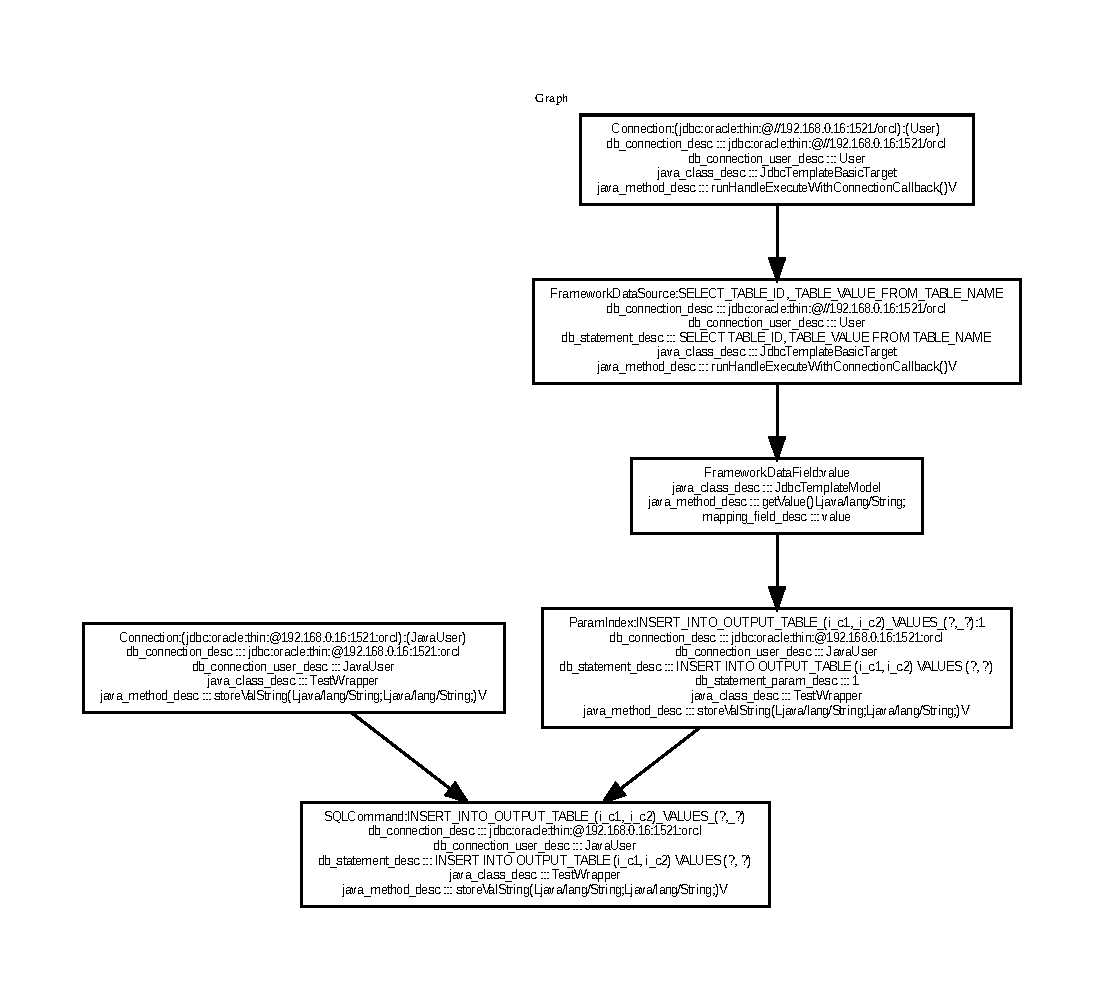
\includegraphics[trim={1cm 1cm 1cm 1.8cm},clip,width=\textwidth]{img/JdbcTemplateBasicTarget-runHandleExecuteWithConnectionCallback.pdf}
  \caption{Visualization of data lineage graph for Spring JDBC Framework}
  \label{results:jdbcTemplate}
\end{figure}

\begin{figure}[h]
  % trim - left lower right upper
  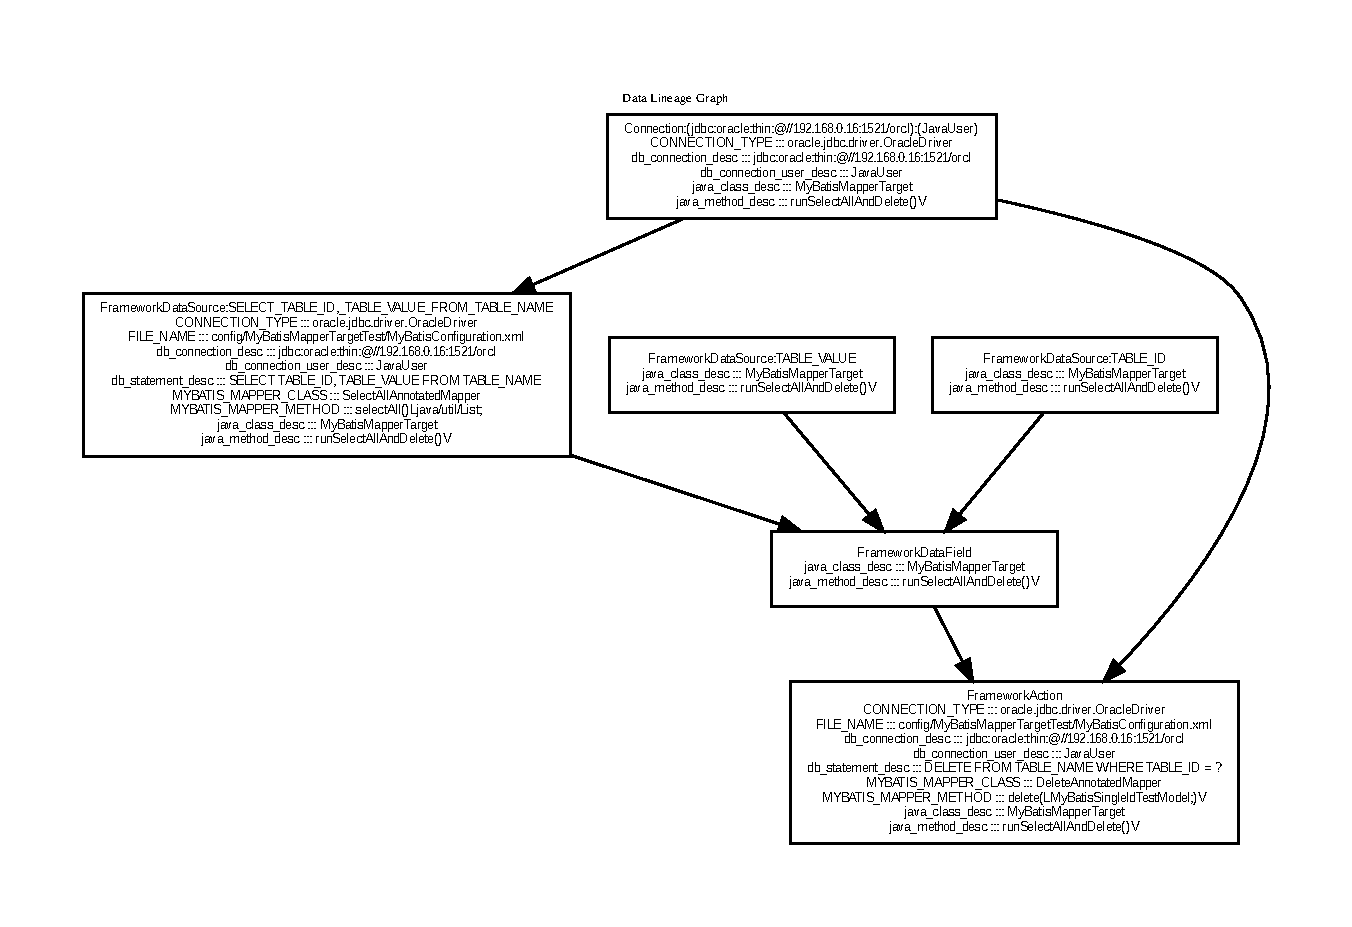
\includegraphics[trim={1cm 1cm 1cm 1.8cm},clip,angle=-90,origin=c,max size={\textwidth}{\textheight}]{img/MyBatisMapperTarget-runSelectAllAndDelete.pdf}
  \caption{Visualization of data lineage graph for MyBatis Framework}
  \label{results:mybatis}
\end{figure}

\begin{figure}[h]
  % trim - left lower right upper
  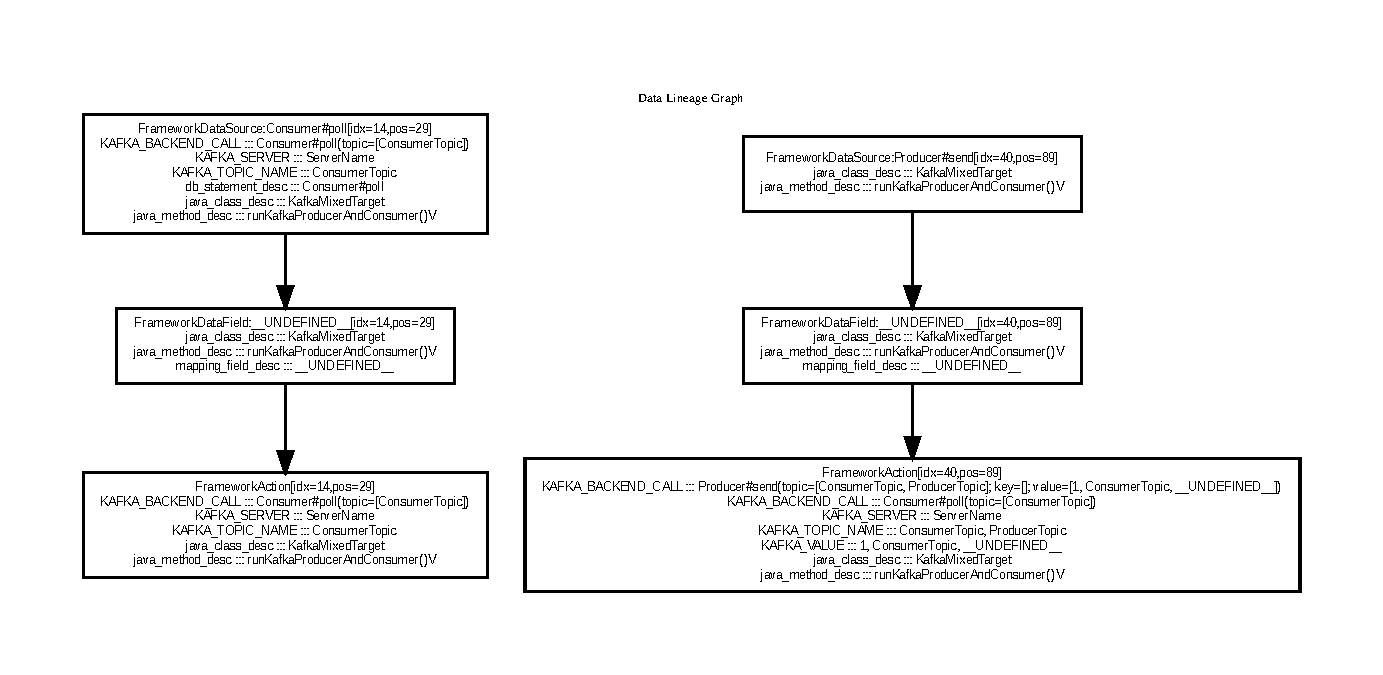
\includegraphics[trim={1cm 1cm 1cm 1.8cm},clip,angle=-90,origin=c,max size={\textwidth}{\textheight}]{img/KafkaMixedTarget-runKafkaProducerAndConsumer.pdf}
  \caption{Visualization of data lineage graph for Kafka Framework}
  \label{results:kafka}
\end{figure}



\section{Limitations of the \ToolName Tool \label{chapter:results:limits}}

There are few limitations of our \ToolName tool.
We point them out in the following list:
\begin{enumerate}
  \item \textbf{Slow data lineage computation.} \\
    The data lineage computation tests in our project last from
    a few tens of seconds to a few minutes. It depends on the
    number of used libraries, their complexity and also from the complexity
    of analysed application.
  \item \textbf{There can be many algorithm iterations until fixpoint is reached.} \\
    The Symbolic analysis library computes method summaries iteratively until
    fixpoint is reached - when there are no changes in the method summaries.
    The number of iterations also depends on the number of methods in the analysed program.
  \item \textbf{Some inaccuracies can occur based on the used\break over-approximation algorithm.} \\
    The Symbolic analysis library computes over-approximate data lineage information (e.g. when accessing
    an element of an array or collection, all elements are considered as output).
  \item \textbf{Disadvantages of static analysis.} \\
    Many disadvantages come with the usage of static analysis
    (e.g. when values are computed dynamically based on the external inputs).
\end{enumerate}



\section{Fulfillment of the Requirements}

In the Section \ref{frameworks:requirements} we pointed out the requirements
on the \ToolName tool to be able to successfully compute the data lineage of
applications that use frameworks for accessing the data.

In the next list we try to explain how the requirements are fulfilled (or not)
by the \ToolName tool:
\begin{enumerate}
  \item \textbf{Analysis of whole Java application.} \\
    Our tool analyses both application and its dependencies
    to distinguish all the data flows. The used WALA framework
    needs all dependencies to create a correct call graph.
  \item \textbf{Identifying the data sources and sinks.} \\
    The plugins for Symbolic analysis library identify the data sources and sinks
    of an analysed application when the corresponding frameworks are used.
  \item \textbf{Correctness, accuracy and efficiency of computing data lineage.} \\
    We explained some limitations of our \ToolName tool in Section \ref{chapter:results:limits}.
    The data lineage computation can take quite long time, depending on the complexity of an analysed
    application and the number of used libraries.
    However, it is expected that analysis of a huge program with many library dependencies
    will run longer than the analysis of other small Java application.
    As the tests in the \ToolName tool show, the data lineage is computed
    in few minutes, therefore the tool is usable in practice.
  \item \textbf{Work with external files.} \\
    The external configuration files are often handled by our plugins for the Symbolic analysis library.
  \item \textbf{Use of concrete values.} \\
    The Symbolic analysis library always tries to resolve actual values of Java primitives and
    \Code{String}s. However, even if in many cases the concrete values cannot be determined,
    the data flow between sources and sinks are preserved.
    As the frameworks often use external files for storing its data, that files can be often read
    by the \ToolName tool to identify the data sources and sinks.
  \item \textbf{Handle callbacks.} \\
    The Symbolic analysis library supports also computing the data flow in callbacks
    from the frameworks to applications.
  \item \textbf{Easy extendability.} \\
    We proposed the pluggable architecture for the Symbolic analysis library.
    We demonstrated the possibilities that result from the changed architecture
    on several library plugins. The plugins identify the data sources and sinks
    of used data processing frameworks.
\end{enumerate}

